\chapter{Week 08}

\section{JROS Profile}

    After much anticipation, the JROS profile has been added to the RWTH JupyterHub. And as expected, the extensions and packages needed to work with ROS were not correctly installed. To elaborate, when a new profile is spawned, neither the \texttt{jupyter-ros} nor the \texttt{jupyterlab-ros} extensions are activated and none of the ROS packages are installed in the default environment.

    This issue was caused because in the \texttt{Dockerfile}, a new conda environment was being created where the extensions and packages were installed but this new environment was never activated. The solution was to install the required packages in the base environment instead.

    Once the packages were installed in the base environment, a newly spawned profile was able to access them. However, a new issue emerged because the ROS commands were not available and none of the ROS environment variables were set. In a local environment, this would indicate that the \texttt{setup.bash} file needed to be sourced before running any ROS commands. But including the sourcing as an instruction in the \texttt{Dockerfile} did not accomplish the desired outcome because that would make the environment variables only available during the building process and they would be reset once the container was running. Further investigation is required to solve these issues.


\section{Gazebo Extension III}

    The development of the Gazebo extension continued starting with fixing the CORB issue encountered last week. The following actions were taken to successfully clear the error:

    \begin{itemize}
        \item A new development environment was created from scratch.
        \item JupyterLab was removed from the base environment and only installed in the development environment. It can become problematic when multiple environments share the same JupyterLab configuration.
    \end{itemize}

    \noindent Additionally, a server was added and configured for the extension. This differs from the Gazebo server which will run as a separate process. When the extension is installed, the server extension should also be enabled.

    \begin{lstlisting}[language=Console]
$ jupyter serverextension enable jupyterlab_gazebo
    \end{lstlisting}

    \subsection{Testing}

    With the Gazebo client, bridge, and server in working condition, it was time to test the models which could be simulated with the extension. There were two ways of accomplishing this, one was to use launch files to spawn specific models and the other way was to add models directly from the client's menu. The first approach failed because the extension still has issues finding the correct path to the model files; it may be necessary to manually reconfigure the assets path when building the client. However, the second approach was successful as seen in Figure~\ref{fig:Boxes}. The same simulation is also shown in Figure~\ref{fig:gazBoxes} with the stand-alone application.

    \begin{figure}[H]
        \centering
        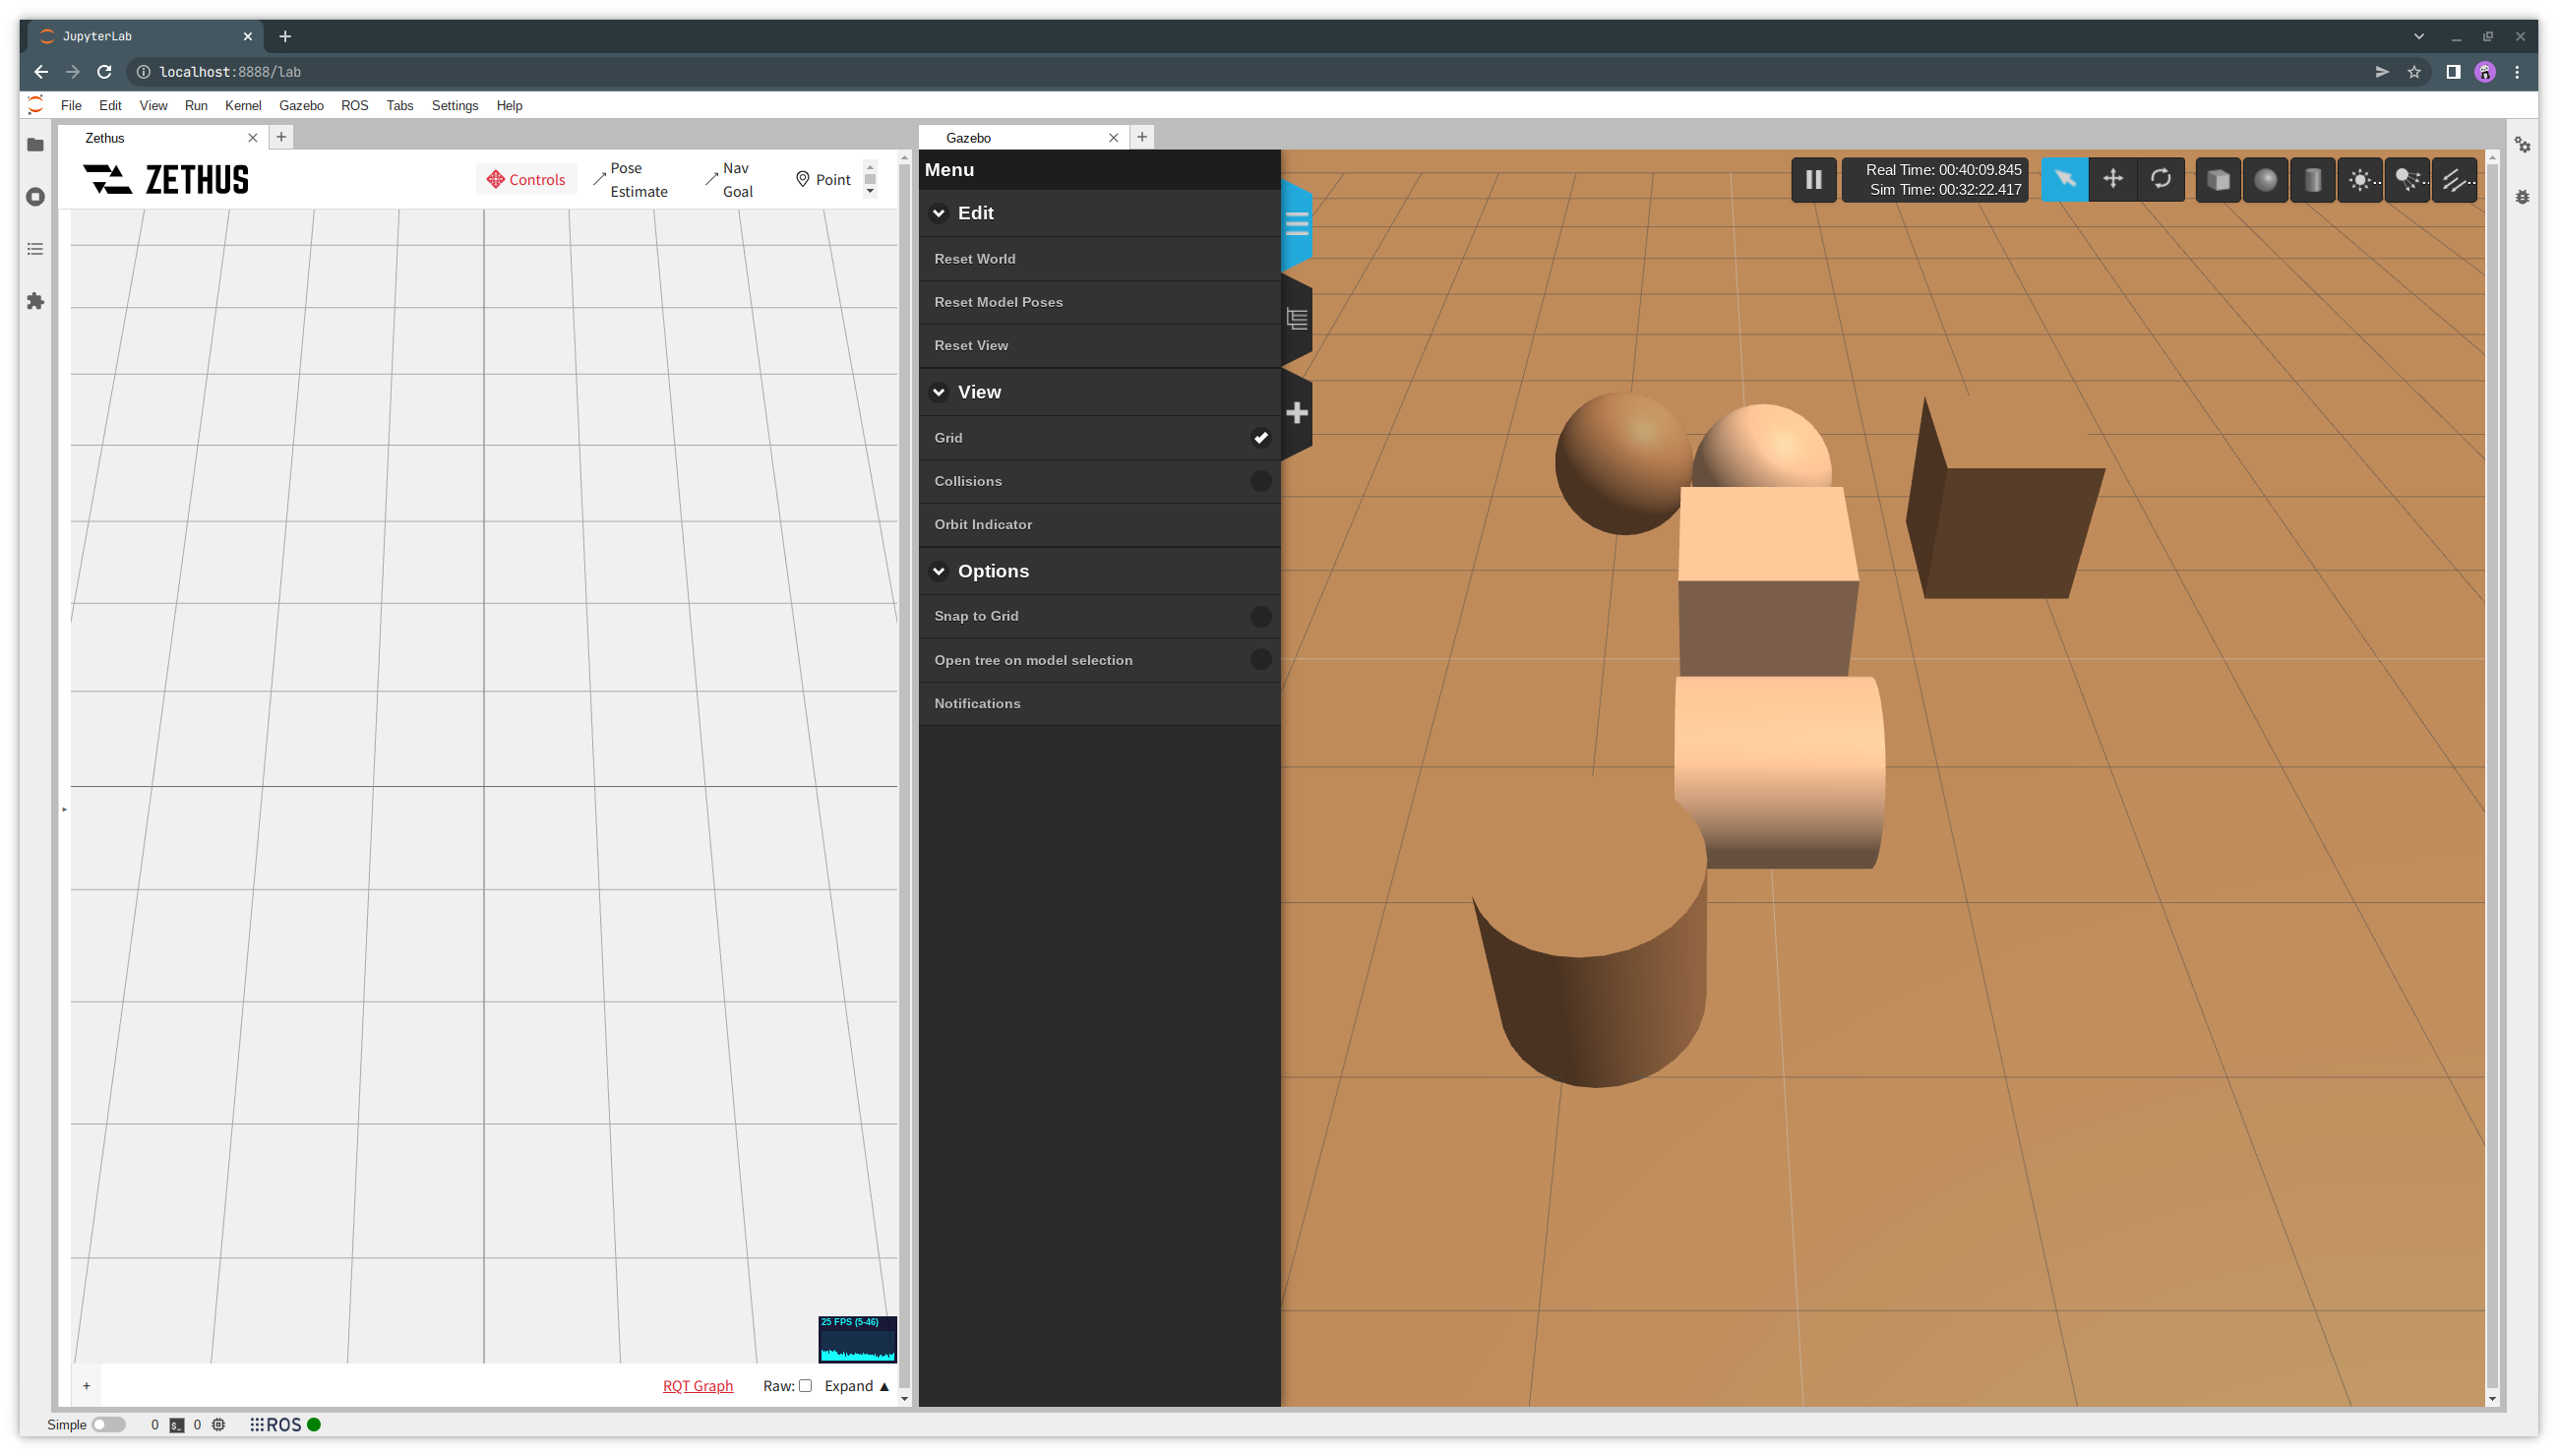
\includegraphics[width=\linewidth]{Images/08_gazExBoxes.png}
        \caption{The Gazebo extension displaying the same shapes the Gazebo server is publishing}
        \label{fig:Boxes}
    \end{figure}

    \begin{figure}[H]
        \centering
        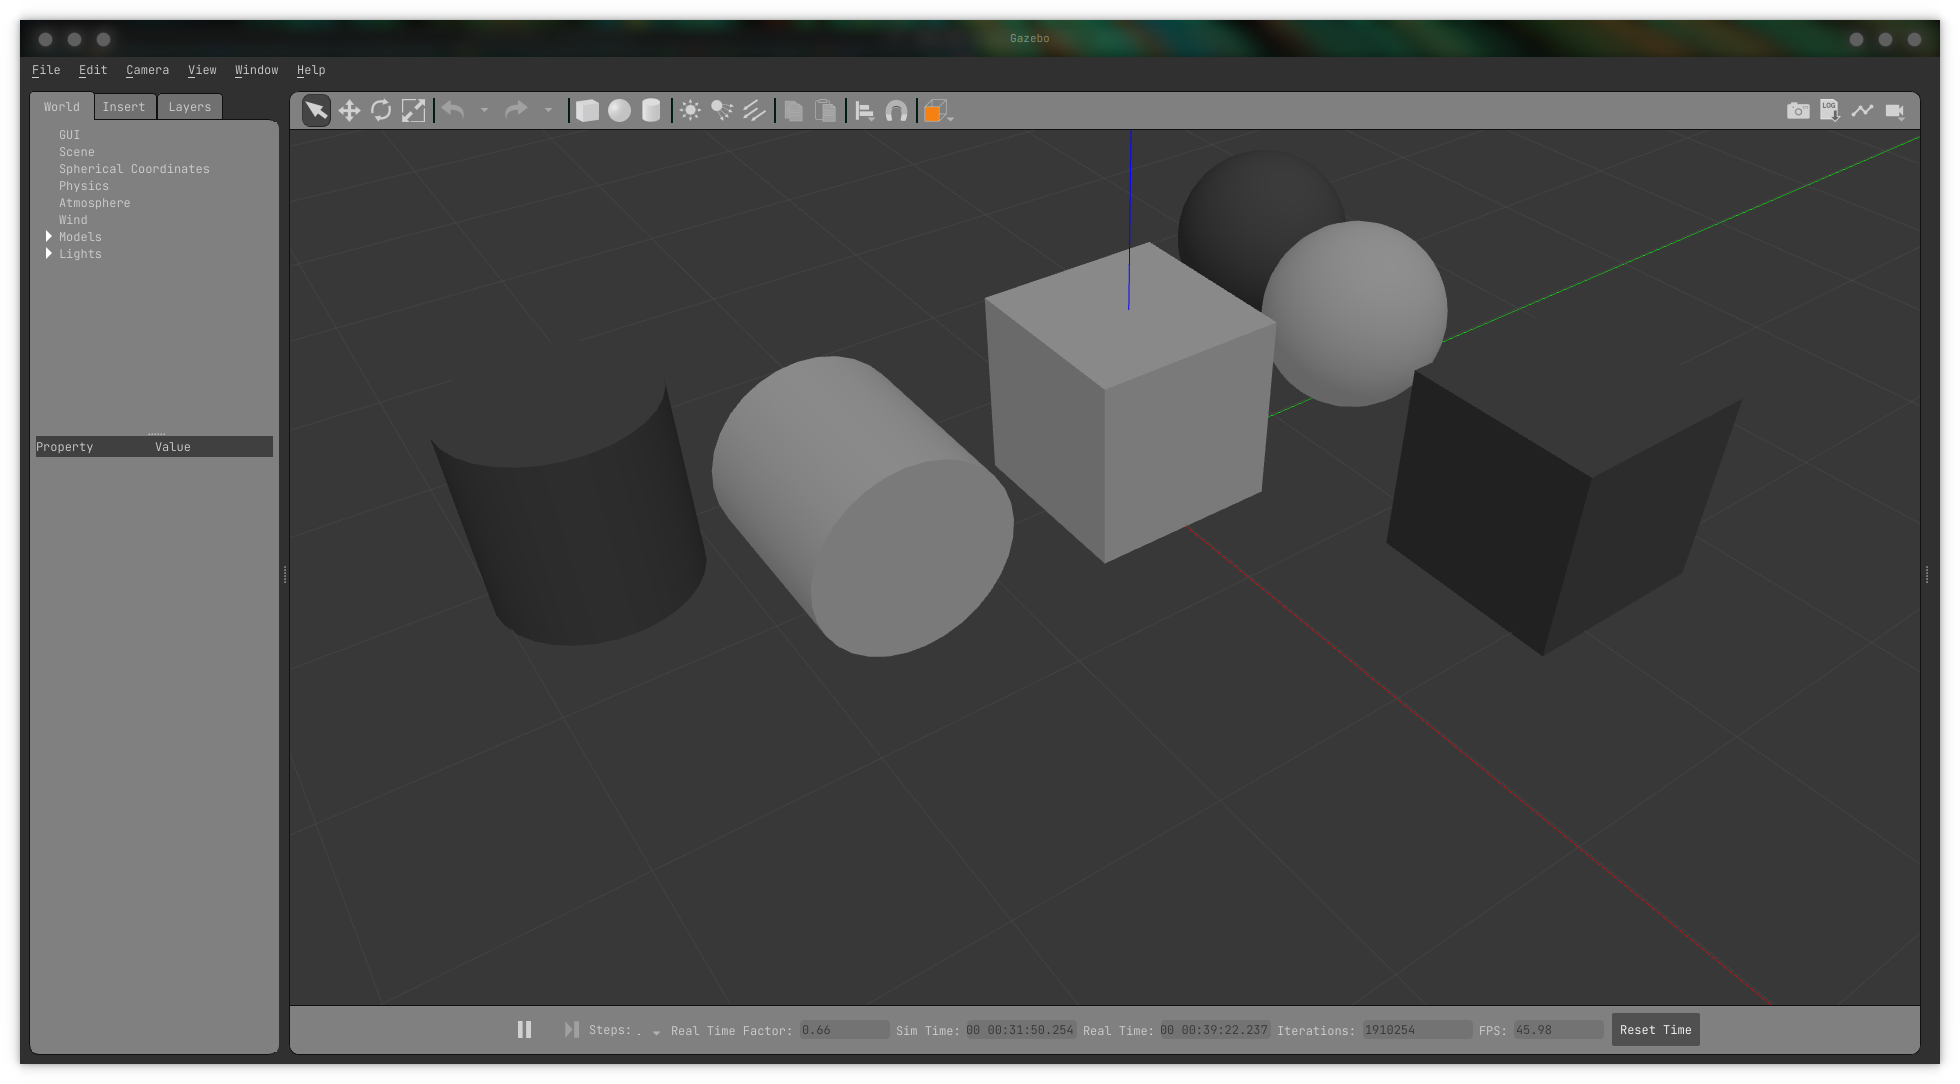
\includegraphics[width=\linewidth]{Images/08_gazAppBoxes.png}
        \caption{The original Gazebo application displaying a variety of shapes}
        \label{fig:gazBoxes}
    \end{figure}
    
\section{Gazebo Ignition}

    The second version of the Gazebo web client was also tested this week. The source code can be found in the \href{https://gitlab.com/ignitionrobotics/web/app/-/tree/gz3d_v2/}{Ignition Robotics GitLab} page. This version can also be accessed on the \href{https://app.gazebosim.org/dashboard}{gazebosim.org} site. In contrast to its predecessor, this application was significantly easier to install since it had been more recently updated. The application can be seen in Figure~\ref{fig:Ignition}. However, the repository is already archived and it is uncertain if the developers plan on continuing with an additional version.

    \begin{figure}[H]
        \centering
        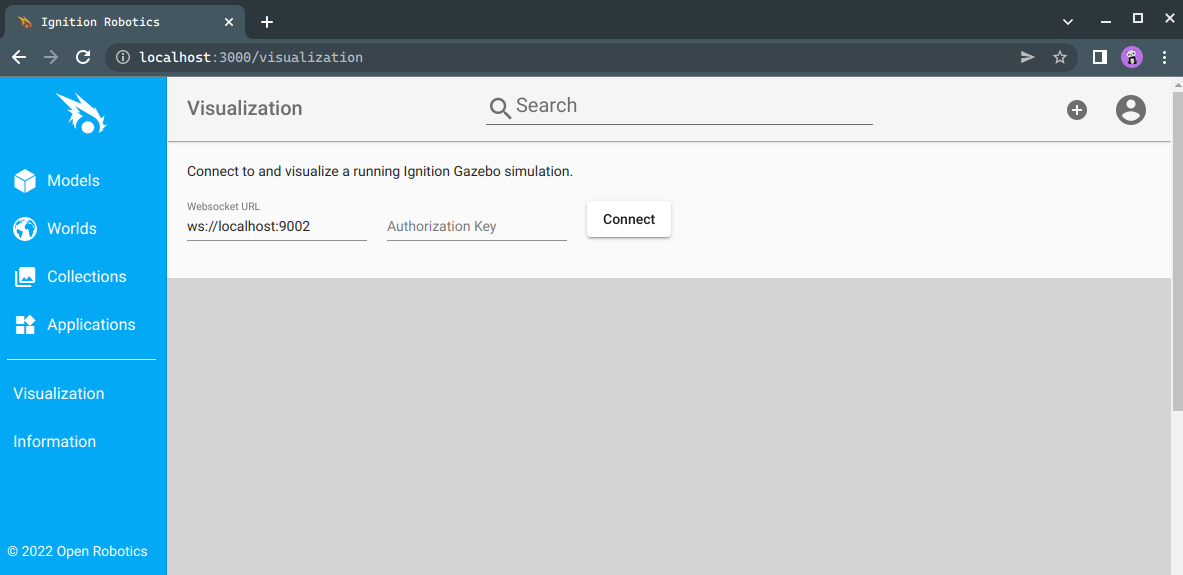
\includegraphics[width=\linewidth]{Images/08_ignition.png}
        \caption{\texttt{gz3d\_v2}, the newest version of the Gazebo web client}
        \label{fig:Ignition}
    \end{figure}



\section{Future Work}

    The development of the Gazebo extension will continue, there are several aspects still left to be accomplished. The main challenges will include configuring the extension so that the Gazebo client and bridge are built automatically during installation. Additionally, when activating the extension, the Gazebo server and bridge should also be launched. And lastly, a more efficient way of installing model files which will also include the robot descriptions from the ROS packages still needs to be determined.